\chapter{Risultati}
\label{cap:risultati}
In questo lavoro di tesi sono stati simulati tre scenari, relativi a tre diverse zone di Roma:
\begin{enumerate}
 \item Il territorio attorno alle facoltà di Ingegneria, Economia e Lettere dell'Università di Roma Tor Vergata.
 \item La zona tra la stazione di Roma Termini e il Colosseo.
 \item L'area con al centro il Pantheon.
\end{enumerate}
Sono state scelte queste tre aree perché presentano una morfologia particolare, partendo dalla zona dell'Università fino a quella 
del Pantheon si può vedere come l'area urbana e la densità di edifici aumenti. Anche le aree verdi passano dalla zona attorno 
all'Università, al Parco Del Colle Oppio, fino alla zona del Pantheon piena di edifici. \\
In tutte le simulazioni l'\ac{UAV} è stato posto al centro dell'area e l'antenna trasmittente è stata supposta un dipolo omnidirezionale. \\
Durante le simulazioni è stata fatta variare la potenza trasmessa dall'apparato \ac{LTE} dell'\ac{UAV} per fare in modo di gestire un 
eventuale risparmio energetico al fine di prolungare la durata della batteria del velivolo. \\
Si ricorda che ogni area ha una superficie di $1km^2$ con una risoluzione di $200 \times 200 pixel$.
Per ognuna di queste tre zone sono stati calcolati questi parametri:
\begin{itemize}
 \item Attenuazione totale, calcolata $pixel \times pixel$.
 \item Raggio medio di copertura.
 \item Raggio medio all'$80^o$ percentile.
\end{itemize}

\section*{Confronto tra le tre zone}
Nella tabella \ref{tab:confrontozone} sono rappresentati i raggi di copertura per ogni zona al variare della potenza, a potenza massima è
molto evidente come il raggio diminuisca con l'aumento della densità urbana.
 \begin{table}[h]\footnotesize
  \caption{Raggi di copertura nelle tre zone al variare della potenza trasmessa.}
  \label{tab:confrontozone}
  \begin{tabularx}{\textwidth}{lXXX}
    \toprule
      & $Ptx = 46dBm$ & $Ptx = 24dBm$ & $Ptx = 20dBm$ \\
    \midrule
      Zona 1 & 506.1867 m & 504.2321 m & 503.3140 m \\
      Zona 2 & 490 m & 392.0459 m & 365.2773 m \\
      Zona 3& 473.0486 m & 408.0747 m & 371.9339 m \\
    \bottomrule
    \end{tabularx}
  \end{table}

\newpage
\section{Area facoltà di Ingegneria, Economia e Lettere}
L'area attorno alle facoltà di Ingegneria, Economia e Lettere dell'Università di Roma Tor Vergata, sono libere da ostacoli.
Gli unici edifici presenti sono quelli dei dipartimenti di Ingegneria (Ingegneria dell'Informazione, Ingegneria Industriale ed Ingegneria
Civile), gli edifici delle facoltà di Lettere e di Economia. 
Il resto, tra parcheggi ed aree verdi, è tutto spazio libero disponibile per l'utente, ci si aspetta quindi che l'area coperta dal segnale
sia la maggior parte se non tutta quanta. \\
Dai calcoli del raggio si ottiene che l'area coperta è circa il $80\%$ di quella totale, ma dato che i calcoli si basano sul calcolo dell'
$80^o$ percentile, risulta che è coperto il $100\%$ dell'area. L'area coperta diminuisce di poco anche a potenza minima.

\begin{figure}[!h]
\centering
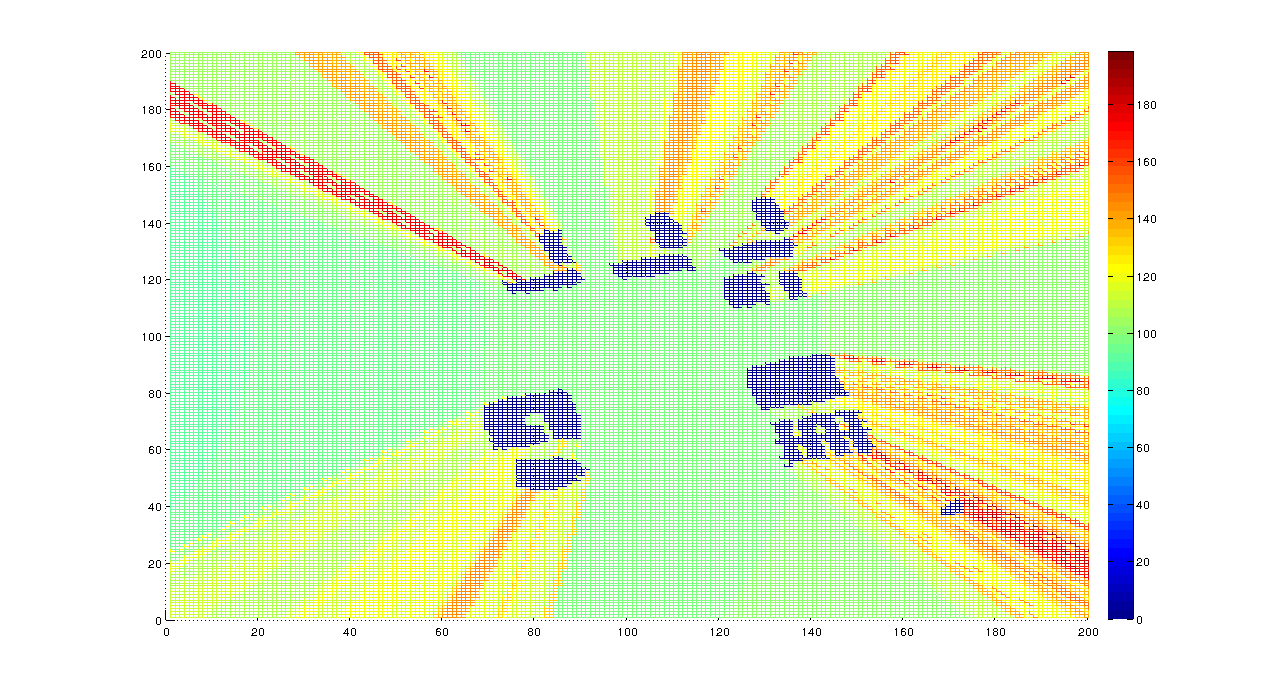
\includegraphics[height=0.5\textwidth]{Immagini/TorVergataIng/attenuazione}
\caption{Attenuazione nella zona delle facoltà di Ingegneria, Economia e Lettere dell'Università di Roma Tor Vergata con potenza
trasmessa pari a $46dBm$. \\
Il raggio medio è pari a $388.3664 m$.\\
Il raggio medio calcolato all'$80^o$ percentile è di $506.1867 m$.}
\label{img:atting}
\end{figure}

\begin{figure}
\centering
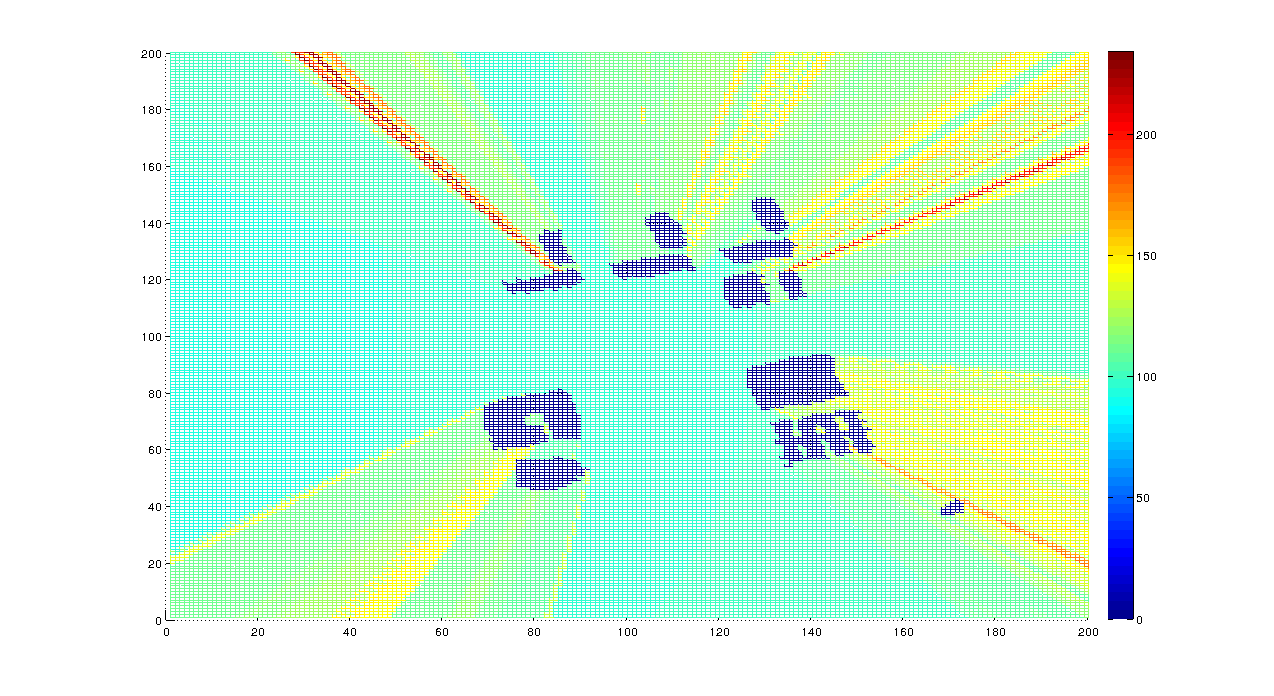
\includegraphics[height=0.5\textwidth]{Immagini/TorVergataIng/attenuazione_pico}
\caption{Attenuazione nella zona delle facoltà di Ingegneria, Economia e Lettere dell'Università di Roma Tor Vergata con potenza
trasmessa pari a $24dBm$. \\
Il raggio medio è pari a $386.0185 m$. \\
Il raggio medio calcolato all'$80^o$ percentile è di $504.2321 m$.}
\label{img:attingpico}
\end{figure}

\begin{figure}
\centering
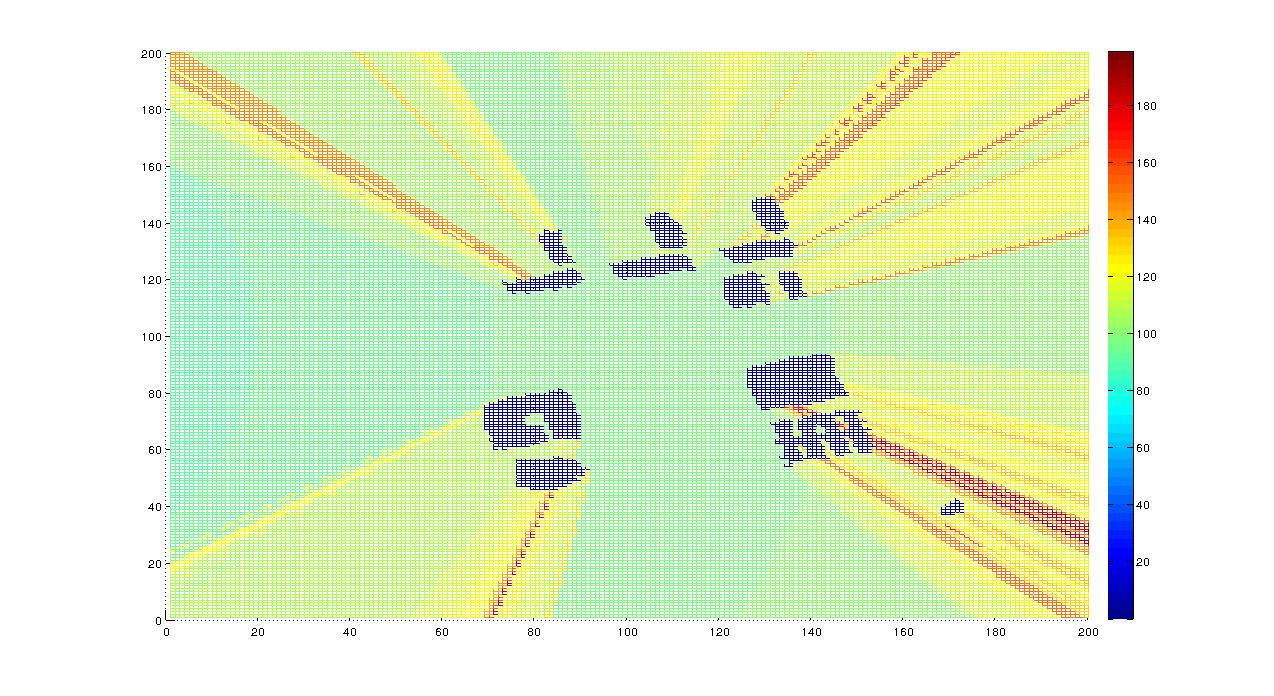
\includegraphics[height=0.5\textwidth]{Immagini/TorVergataIng/attenuazione_femto}
\caption{Attenuazione nella zona delle facoltà di Ingegneria, Economia e Lettere dell'Università di Roma Tor Vergata con potenza
trasmessa pari a $20dBm$. \\
Il raggio medio è pari a $384.704 m$. \\
Il raggio medio calcolato all'$80^o$ percentile è di $503.3140 m$.}
\label{img:attingfemto}
\end{figure}

\newpage
\section{Area tra Roma Termini e Colosseo}
Nella zona tra la stazione di Roma Termini e il Colosseo l'ambiente è una via di mezzo tra urbano e spazio libero, si va dal Parco Del
Colle Oppio fino alla zona urbana attorno a Roma Termini. \\
Con la massima potenza trasmessa si riesce a coprire il $75\%$ dell'area, quindi sempre riferendosi al percentile $80$ si capisce che la
copertura è quasi totale, a potenza minima, invece, la copertura scende al $40\%$ quindi l'area coperta è circa il $50\%$.

\begin{figure}[!h]
\centering
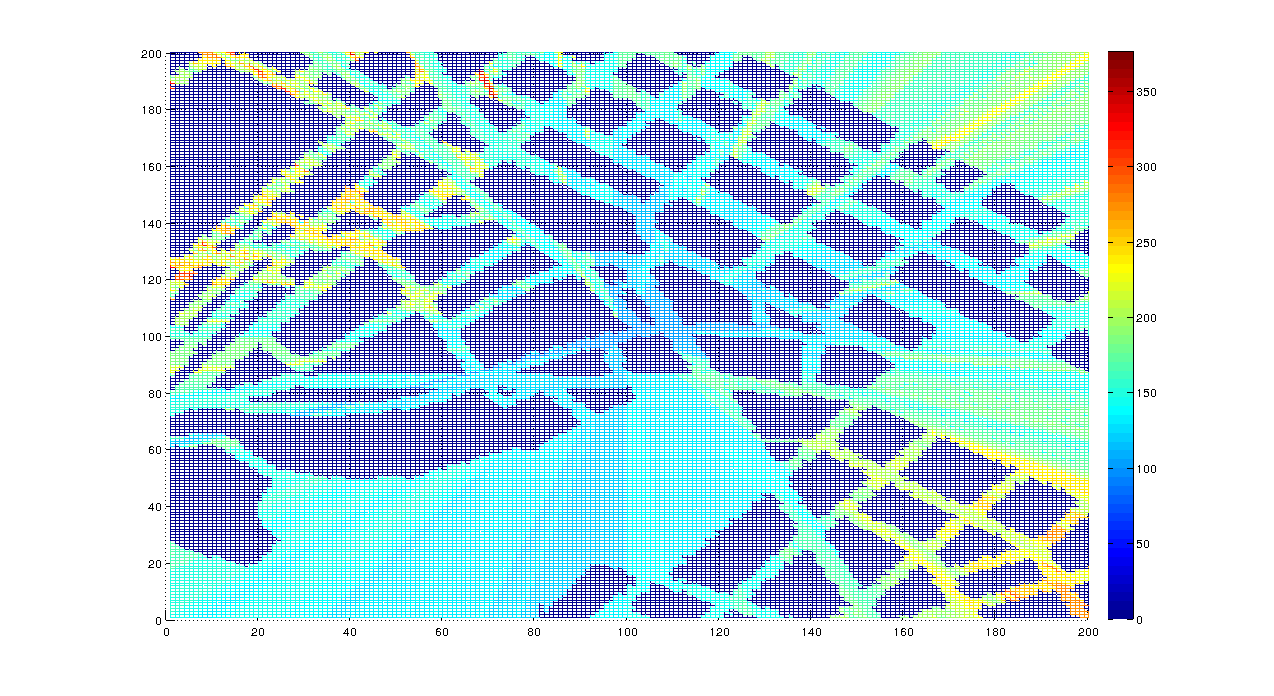
\includegraphics[height=0.5\textwidth]{Immagini/ColleOppio/attenuazione}
\caption{Attenuazione nella zona tra Colle Oppio e Roma Termini con potenza trasmessa pari a $46dBm$. \\
Il raggio medio è pari a $363.9597 m$.\\
Il raggio medio calcolato all'$80^o$ percentile è di $490 m$.}
\label{img:attcolleoppio}
\end{figure}

\begin{figure}
\centering
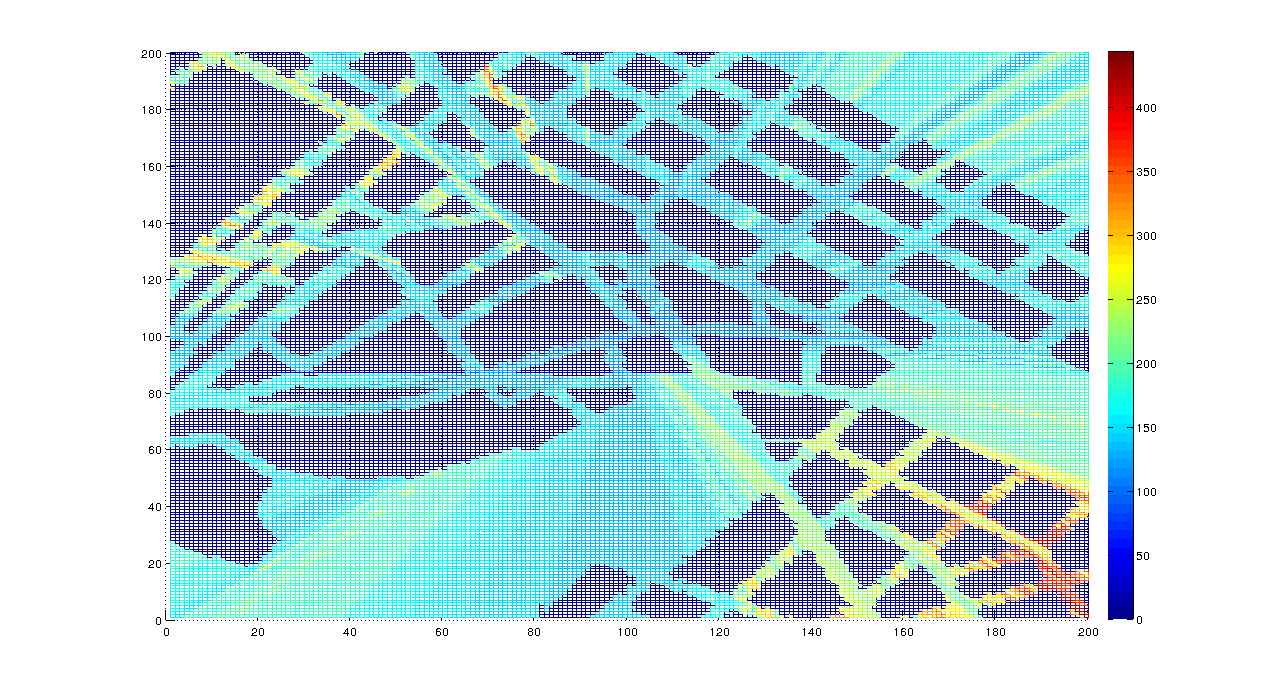
\includegraphics[height=0.5\textwidth]{Immagini/ColleOppio/attenuazione_pico}
\caption{Attenuazione nella zona tra Colle Oppio e Roma Termini con potenza trasmessa pari a $24dBm$. \\
Il raggio medio è pari a $282.0619 m$.\\
Il raggio medio calcolato all'$80^o$ percentile è di $392.0459 m$.}
\label{img:attcolleoppiopico}
\end{figure}

\begin{figure}
\centering
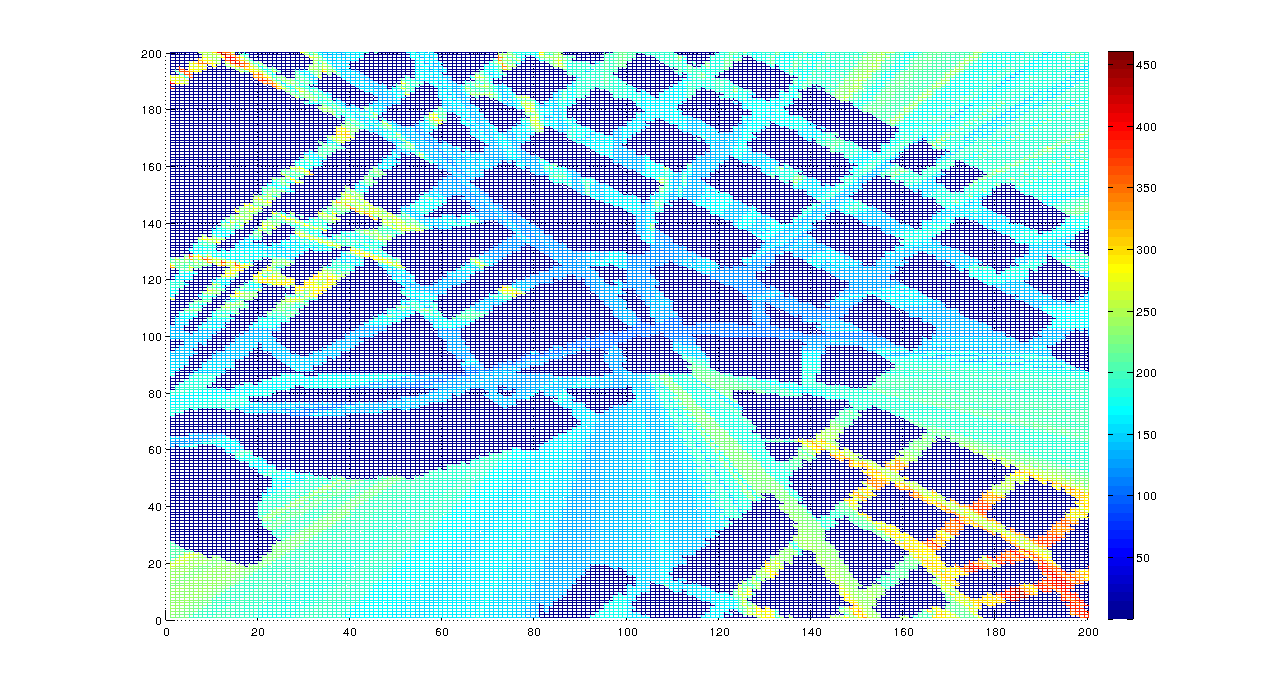
\includegraphics[height=0.5\textwidth]{Immagini/ColleOppio/attenuazione_femto}
\caption{Attenuazione nella zona tra Colle Oppio e Roma Termini con potenza trasmessa pari a $20dBm$. \\
Il raggio medio è pari a $256.2801 m$.\\
Il raggio medio calcolato all'$80^o$ percentile è di $365.2773 m$.}
\label{img:attcolleoppiofemto}
\end{figure}

\newpage
\section{Area Pantheon}
Nell'area urbana dove è ubicato il Pantheon, l'ambiente urbano è predominante è quello urbano, non ci sono aree libere e l'utente può
trovarsi solo lungo le strade. \\
A potenza massima il raggio all'$80^o$ percentile copre un'area pari al $70\%$, normalizzando si ottiene che l'area coperta è circa 
l'$87\%$, al diminuire della potenza l'area normalizzata coperta arriva a circa un $55\%$

\begin{figure}[!h]
\centering
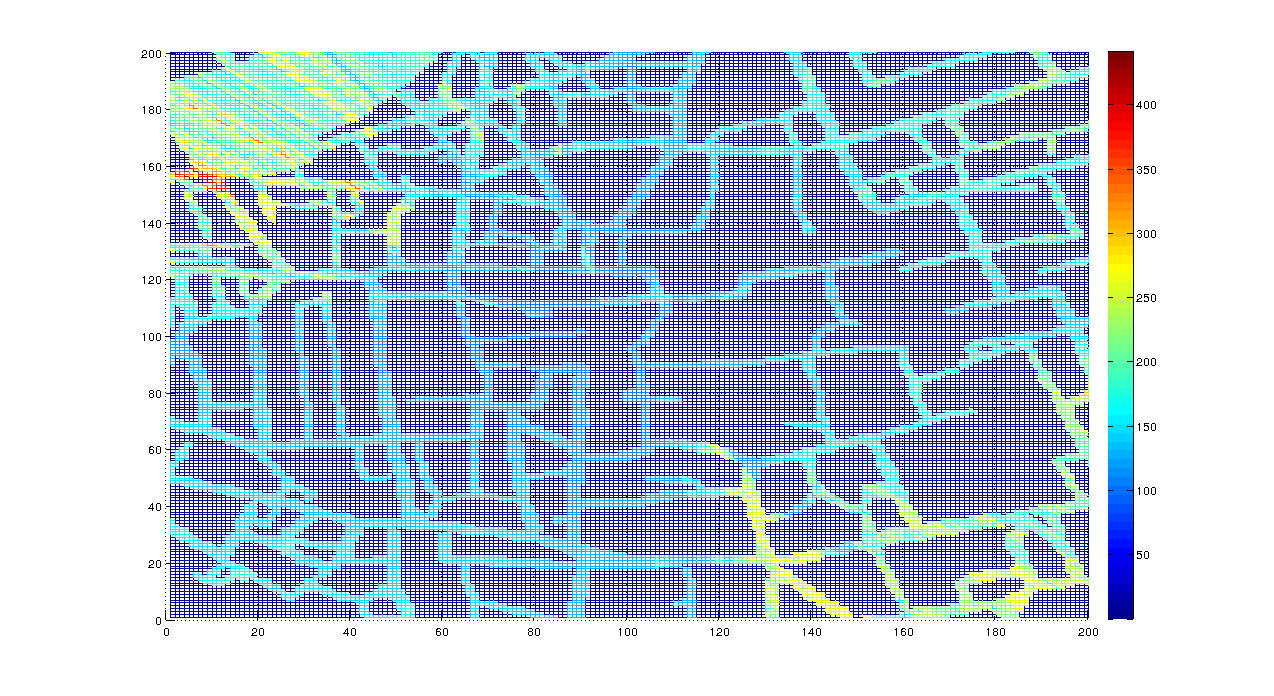
\includegraphics[height=0.5\textwidth]{Immagini/Pantheon/attenuazione}
\caption{Attenuazione nell'area del Pantheon con potenza trasmessa pari a $46dBm$. \\
Il raggio medio è pari a $348.2113 m$.\\
Il raggio medio calcolato all'$80^o$ percentile è di $473.0486 m$.}
\label{img:attpantheon}
\end{figure}

\begin{figure}
\centering
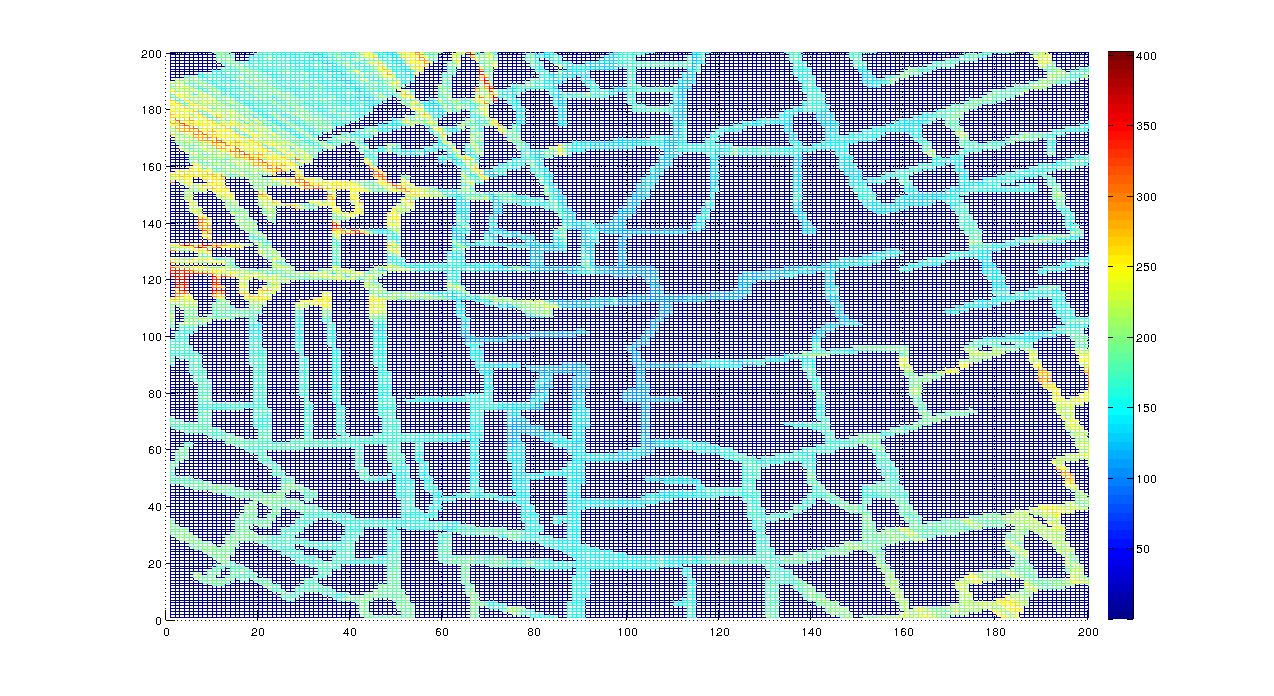
\includegraphics[height=0.5\textwidth]{Immagini/Pantheon/attenuazione_pico}
\caption{Attenuazione nell'area del Pantheon con potenza trasmessa pari a $24dBm$. \\
Il raggio medio è pari a $294.3916 m$.\\
Il raggio medio calcolato all'$80^o$ percentile è di $408.0747 m$.}
\label{img:attpantheonpico}
\end{figure}

\begin{figure}
\centering
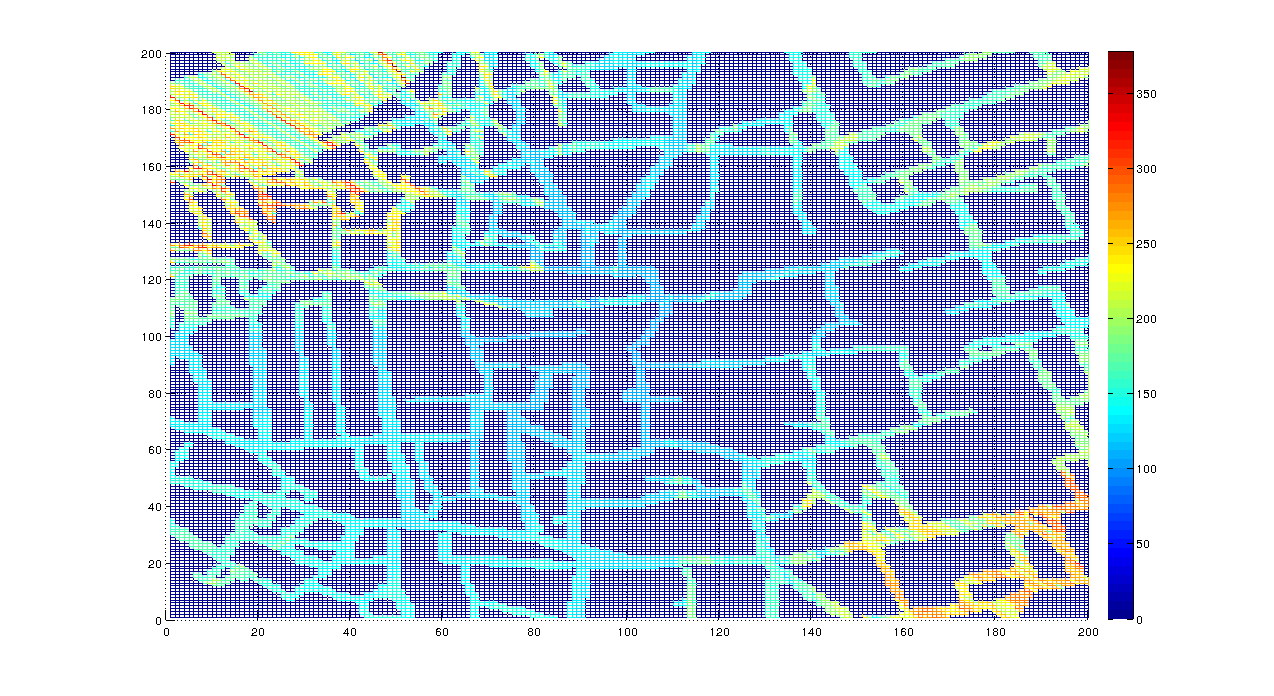
\includegraphics[height=0.5\textwidth]{Immagini/Pantheon/attenuazione_femto}
\caption{Attenuazione nell'area del Pantheon con potenza trasmessa pari a $20dBm$. \\
Il raggio medio è pari a $242.1427 m$.\\
Il raggio medio calcolato all'$80^o$ percentile è di $371.9339 m$.}
\label{img:attpantheonfemto}
\end{figure}